%!TEX root = Main.tex
\documentclass[Main]{subfiles}

\begin{document}

\section{Design And Implementation} % (fold)
\label{sec:design_and_implementation}

	\subsection{Data Input} % (fold)
	\label{sub:data_input}

		The MATLAB script \texttt{InputData.m} uses build in functions to extract data from the downloaded G1SST database.
		It takes as input an upper and lower bound and an eastern and western bound in between which it is supposed to a square set of data.

		The data is converted from Kelvin to Celsius, to make it more semantically understandable.
		The data is then saved to a \texttt{.mat}-file for use in other scripts.

		Finally the data is shown on a colored contour-plot (see Figure \ref{fig:ExampleSSTData}), for illustration and inspection purposes.

	
		% subsection data_input (end)

	\subsection{Sparsity Estimation} % (fold)
	\label{sub:sparsity_estimation}

		The MATLAB script \texttt{EvalSparsity.m} takes as input to \emph{.mat}-file described in Section \ref{sub:data_input}.

		It vectorizes the data map by stacking either the rows or the columns.
		The snake pattern, described in Section \ref{par:vectorization_of_data_map} is also implemented, and is enabled by a boolean \texttt{snake}.

		Then it evaluates the sparsity by taking either the DFT or the DCT of the signal.
		The sparsity is the number, $k$, of coefficients greater than 10 or 0.1, respectively.
		It then tries to do a reconstruction using $M = 6*k$ randomly selected samples, and calculates the normalized error:
		%
		\begin{equation}
			e_{normalized} = \frac
				{\|\mathbf{\hat{u}}(n) - \mathbf{u}(n)\|_{l2}}
				{\|\mathbf{u}(n)\|_{l2}}
		\end{equation}

		In Figure \ref{fig:ExEvalSparseSnakeOff} below the result of running the script on data from a patch of the North Sea.
		The data is visibly sparse, in the sense that most of the energy in the DCT is confined to at small number of coefficients.
		The power does however not taper off as rapidly as one would like.
		Especially, there are some powerful harmonics present.
		A suggestion for reducing these were presented in Section \ref{par:vectorization_of_data_map} and will be tested in Section \ref{sub:comparison_of_suggested_methods}.

		Another way of determining the sufficient number of samples, $N_S$ required for reconstruction is by doing is experimentally.
		This process entails attempting reconstruction with an increasing number of samples available, and seeing when the error has decreased enough.

		The MATLAB script \texttt{FindOptimumNs.m} does this.
		It goes trough the process of reconstructing the data from randomly selected data points, for a series of logarithmically spaced values of $M$, doing it 10 times for each value and averaging the result.
		This produces a plot like the on shown in \fxnote{insert optimum Ns figure here}.
		This figure can then be used to give a good estimate of $N_s$.

		\begin{figure}[H]
			\centering 
			\includegraphics[width=\textwidth]{ExEvalSparseSnakeOff.eps}
			\caption{
				Results of running \texttt{EvalSparsity.m} on a patch of data from the North Sea.}
			\label{fig:ExEvalSparseSnakeOff}
		\end{figure}

		\begin{figure}[H]
			\centering 
			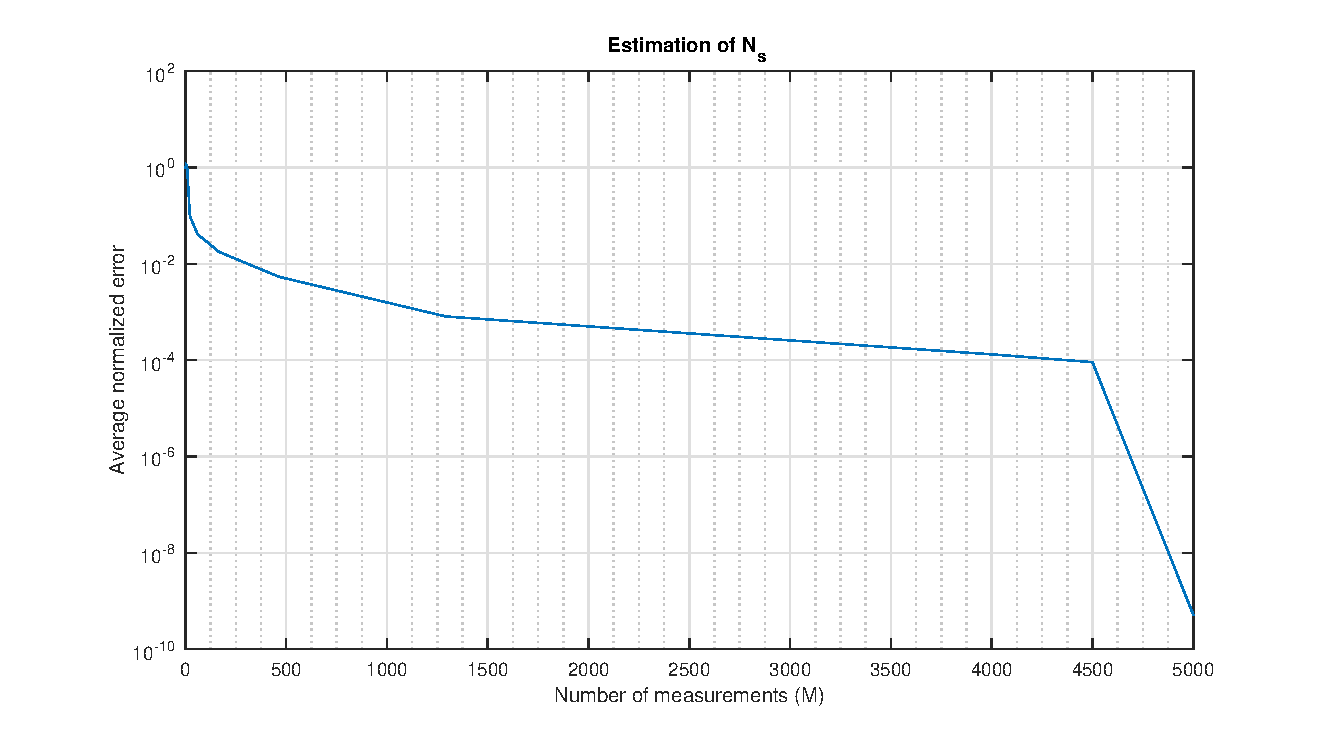
\includegraphics[width=\textwidth]{FindOptimumNsSnakeOff.eps}
			\caption{
				Results of running \texttt{FindOptimumNs.m} on a patch of data from the North Sea. As can be seen from the figure, a $N_s \approx 3300$ is sufficient, consistent with results above.}
			\label{fig:FindOptimumNsSnakeOff}
		\end{figure}



	
		% subsection sparsity_estimation (end)

	\subsection{Estimaton of $q_s$ and $p_s$} % (fold)
	\label{sub:estimaton_of_q_s_and_p_s_}

		With an estimate of $N_s$, you can now calculate the required sensing probability, $p_s$.
	
		% subsection estimaton_of_q_s_and_p_s_ (end)

	\subsection{Simulation of Random Access Transmission} % (fold)
	\label{sub:simulation_of_random_access_transmission}



		\fxnote{Mean K vs p figure}
		\fxnote{reconstruction error vs p figure}
	
		% subsection simulation_of_random_access_transmission (end)

	\subsection{Data Reconstruction (Sensor Fusion)} % (fold)
	\label{sub:data_reconstruction}
	
		% subsection data_reconstruction (end)

	
	\subsection{Comparison of Suggested Methods} % (fold)
	\label{sub:comparison_of_suggested_methods}

		\fxnote{comparison of signal and DCT with and without snake}
	
		% subsection comparison_of_suggested_methods (end)

	% section design_and_implementation (end)


\end{document}